\normalfalse \difficiletrue \tdifficilefalse
\correctionfalse

%\UPSTIidClasse{11} % 11 sup, 12 spé
%\newcommand{\UPSTIidClasse}{11}

\exer{Pèse camion  $\star$ \label{C2:07:57:02}}
\setcounter{numques}{0}
\UPSTIcompetence[2]{C2-07}
\index{Compétence C2-07}
\index{PFS}
\index{Pèse camion}
\ifcorrection
\else
\textbf{Pas de corrigé pour cet exercice.}
\fi

\ifprof
\else
On considère un bâti \textbf{0} auquel est attaché le repère$\mathcal{R}=\left(O;\vect{x_0};\vect{y_0};\vect{z_0} \right)$. Le champ de pesanteur est $g=-g\vect{y_0}$.La barre \textbf{1} est liée au bâti \textbf{0} par une liaison pivot parfaite d’axe $\left(A,\vect{z_0}\right)$. Le plateau porte camion \textbf{2} est lié à la barre \textbf{1} par une liaison pivot parfaite d’axe $\left(C,\vect{z_0}\right)$. Le levier \textbf{3} est lié au bâti \textbf{0} par une liaison pivot parfaite d’axe $\left(B,\vect{z_0}\right)$. Ce levier est également lié au plateau \textbf{2} par une liaison pivot parfaite d’axe $\left(D,\vect{z_0}\right)$. Le camion \textbf{4}, de centre de masse $G$ et de masse $M$ inconnue, repose sur le plateau \textbf{2}.
L’action mécanique connue est caractérisée par : $\{\text{ext}\rightarrow 3\}=\left\{
\begin{array}{c}
-F\vect{y_0} \\
\vect{0} \\
\end{array}
\right\}_E$ .


\begin{center}
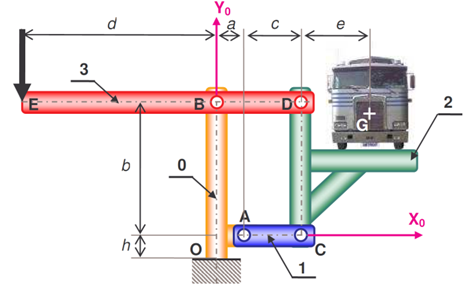
\includegraphics[width=\linewidth]{57_01}
\end{center}


\fi

\question{Tracer le graphe des liaisons en indiquant les actions mécaniques. }
\ifprof
\begin{center}
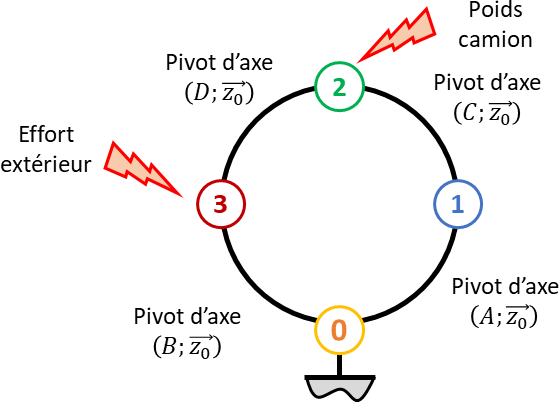
\includegraphics[width=.5\linewidth]{57_01_c}
\end{center}
\else
\fi



\question{Appliquer le PFS au solide 1.}
\ifprof
\else
\fi


\question{Appliquer le PFS au solide 2.}
\ifprof
\else
\fi


\question{Appliquer le PFS au solide 3.}
\ifprof
\else
\fi


\question{Déterminer les actions mécaniques dans chacune des liaisons.}
\ifprof
\else
\fi

\ifprof
\else
\begin{flushright}
\footnotesize{Corrigé voir \ref{C2:07:57:02}.}
\end{flushright}%
\fi